\documentclass[a4paper]{article}
\usepackage{graphicx}

\usepackage[utf8]{inputenc}
\usepackage[a4paper]{geometry}
%\usepackage[]{algorithm2e}
\usepackage{amsfonts}
\usepackage{amsmath}
\usepackage{mathtools}
\usepackage{array}
\usepackage[francais]{babel}

\title{Informatique Embarqué}
\author{Thomas Salmon}
\date{07/02/2014}

\begin{document}

Mes choix:

Etant donné que l'on doit se résoudre a recevoir un tableau de 2 dimension en paramètre, j'ai opté de travailler sur un tableau a une seule dimension afin de pouvoir renvoyer le résultat des opérations.

Voici un apercu du fonctionnement de la fonction:
Pour remplir un tel tableau:

\begin{tabular}{|*{4}{c|}}
    \hline
     1  & 2  & 3  & 4 \\
    \hline
     10 & 11 & 12 & 5 \\
    \hline
     9  & 8  & 7  & 6\\
    \hline
\end{tabular}

On le représente comme ceci

\begin{tabular}{|*{12}{c|}}
    \hline
     1  & 2  & 3  & 4 & 10 & 11 & 12 & 5 & 9  & 8  & 7  & 6\\
    \hline
\end{tabular}

L'algorithme est constitué de 4 boucles successives:

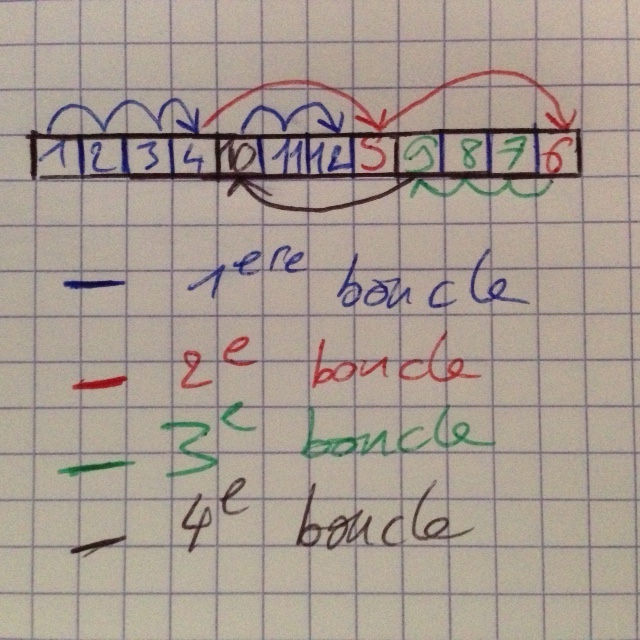
\includegraphics[width=4in]{algo}

Tout d'abord, on rempli case par case jusqu'a ce qu'on ait fait une ligne, puis on saute de colonnes en colonnes jusqu'a la derniere case, ensuite on revient sur nos pas jusqu'a faire une nouvelle ligne, on remonte colonne par colonne jusqu'a revenir a point de départ, et on recommence jusqu'a ce que notre compteur de case ai atteint le nombre ligne * colonne

J'ai consacré 2 heures par jour à ce travail

Je n'ai soumis mon travail a aucun groupe

\end{document}